% Options for packages loaded elsewhere
\PassOptionsToPackage{unicode}{hyperref}
\PassOptionsToPackage{hyphens}{url}
%
\documentclass[
]{article}
\usepackage{lmodern}
\usepackage{amssymb,amsmath}
\usepackage{ifxetex,ifluatex}
\ifnum 0\ifxetex 1\fi\ifluatex 1\fi=0 % if pdftex
  \usepackage[T1]{fontenc}
  \usepackage[utf8]{inputenc}
  \usepackage{textcomp} % provide euro and other symbols
\else % if luatex or xetex
  \usepackage{unicode-math}
  \defaultfontfeatures{Scale=MatchLowercase}
  \defaultfontfeatures[\rmfamily]{Ligatures=TeX,Scale=1}
\fi
% Use upquote if available, for straight quotes in verbatim environments
\IfFileExists{upquote.sty}{\usepackage{upquote}}{}
\IfFileExists{microtype.sty}{% use microtype if available
  \usepackage[]{microtype}
  \UseMicrotypeSet[protrusion]{basicmath} % disable protrusion for tt fonts
}{}
\makeatletter
\@ifundefined{KOMAClassName}{% if non-KOMA class
  \IfFileExists{parskip.sty}{%
    \usepackage{parskip}
  }{% else
    \setlength{\parindent}{0pt}
    \setlength{\parskip}{6pt plus 2pt minus 1pt}}
}{% if KOMA class
  \KOMAoptions{parskip=half}}
\makeatother
\usepackage{xcolor}
\IfFileExists{xurl.sty}{\usepackage{xurl}}{} % add URL line breaks if available
\IfFileExists{bookmark.sty}{\usepackage{bookmark}}{\usepackage{hyperref}}
\hypersetup{
  pdfauthor={Pulan Yu},
  hidelinks,
  pdfcreator={LaTeX via pandoc}}
\urlstyle{same} % disable monospaced font for URLs
\usepackage[margin=1in]{geometry}
\usepackage{color}
\usepackage{fancyvrb}
\newcommand{\VerbBar}{|}
\newcommand{\VERB}{\Verb[commandchars=\\\{\}]}
\DefineVerbatimEnvironment{Highlighting}{Verbatim}{commandchars=\\\{\}}
% Add ',fontsize=\small' for more characters per line
\usepackage{framed}
\definecolor{shadecolor}{RGB}{248,248,248}
\newenvironment{Shaded}{\begin{snugshade}}{\end{snugshade}}
\newcommand{\AlertTok}[1]{\textcolor[rgb]{0.94,0.16,0.16}{#1}}
\newcommand{\AnnotationTok}[1]{\textcolor[rgb]{0.56,0.35,0.01}{\textbf{\textit{#1}}}}
\newcommand{\AttributeTok}[1]{\textcolor[rgb]{0.77,0.63,0.00}{#1}}
\newcommand{\BaseNTok}[1]{\textcolor[rgb]{0.00,0.00,0.81}{#1}}
\newcommand{\BuiltInTok}[1]{#1}
\newcommand{\CharTok}[1]{\textcolor[rgb]{0.31,0.60,0.02}{#1}}
\newcommand{\CommentTok}[1]{\textcolor[rgb]{0.56,0.35,0.01}{\textit{#1}}}
\newcommand{\CommentVarTok}[1]{\textcolor[rgb]{0.56,0.35,0.01}{\textbf{\textit{#1}}}}
\newcommand{\ConstantTok}[1]{\textcolor[rgb]{0.00,0.00,0.00}{#1}}
\newcommand{\ControlFlowTok}[1]{\textcolor[rgb]{0.13,0.29,0.53}{\textbf{#1}}}
\newcommand{\DataTypeTok}[1]{\textcolor[rgb]{0.13,0.29,0.53}{#1}}
\newcommand{\DecValTok}[1]{\textcolor[rgb]{0.00,0.00,0.81}{#1}}
\newcommand{\DocumentationTok}[1]{\textcolor[rgb]{0.56,0.35,0.01}{\textbf{\textit{#1}}}}
\newcommand{\ErrorTok}[1]{\textcolor[rgb]{0.64,0.00,0.00}{\textbf{#1}}}
\newcommand{\ExtensionTok}[1]{#1}
\newcommand{\FloatTok}[1]{\textcolor[rgb]{0.00,0.00,0.81}{#1}}
\newcommand{\FunctionTok}[1]{\textcolor[rgb]{0.00,0.00,0.00}{#1}}
\newcommand{\ImportTok}[1]{#1}
\newcommand{\InformationTok}[1]{\textcolor[rgb]{0.56,0.35,0.01}{\textbf{\textit{#1}}}}
\newcommand{\KeywordTok}[1]{\textcolor[rgb]{0.13,0.29,0.53}{\textbf{#1}}}
\newcommand{\NormalTok}[1]{#1}
\newcommand{\OperatorTok}[1]{\textcolor[rgb]{0.81,0.36,0.00}{\textbf{#1}}}
\newcommand{\OtherTok}[1]{\textcolor[rgb]{0.56,0.35,0.01}{#1}}
\newcommand{\PreprocessorTok}[1]{\textcolor[rgb]{0.56,0.35,0.01}{\textit{#1}}}
\newcommand{\RegionMarkerTok}[1]{#1}
\newcommand{\SpecialCharTok}[1]{\textcolor[rgb]{0.00,0.00,0.00}{#1}}
\newcommand{\SpecialStringTok}[1]{\textcolor[rgb]{0.31,0.60,0.02}{#1}}
\newcommand{\StringTok}[1]{\textcolor[rgb]{0.31,0.60,0.02}{#1}}
\newcommand{\VariableTok}[1]{\textcolor[rgb]{0.00,0.00,0.00}{#1}}
\newcommand{\VerbatimStringTok}[1]{\textcolor[rgb]{0.31,0.60,0.02}{#1}}
\newcommand{\WarningTok}[1]{\textcolor[rgb]{0.56,0.35,0.01}{\textbf{\textit{#1}}}}
\usepackage{graphicx,grffile}
\makeatletter
\def\maxwidth{\ifdim\Gin@nat@width>\linewidth\linewidth\else\Gin@nat@width\fi}
\def\maxheight{\ifdim\Gin@nat@height>\textheight\textheight\else\Gin@nat@height\fi}
\makeatother
% Scale images if necessary, so that they will not overflow the page
% margins by default, and it is still possible to overwrite the defaults
% using explicit options in \includegraphics[width, height, ...]{}
\setkeys{Gin}{width=\maxwidth,height=\maxheight,keepaspectratio}
% Set default figure placement to htbp
\makeatletter
\def\fps@figure{htbp}
\makeatother
\setlength{\emergencystretch}{3em} % prevent overfull lines
\providecommand{\tightlist}{%
  \setlength{\itemsep}{0pt}\setlength{\parskip}{0pt}}
\setcounter{secnumdepth}{-\maxdimen} % remove section numbering

\author{Pulan Yu}
\date{2/24/2020}

\begin{document}

\hypertarget{part-1-simulation}{%
\subsection{Part 1 Simulation}\label{part-1-simulation}}

In this section, the exponential distribution in R will be investigated
and compared with the Central Limit Theorem.

The exponential distribution will be simulated in R with rexp(n, lambda)
where lambda is the rate parameter. The mean of exponential distribution
is 1/lambda and the standard deviation is also 1/lambda. lambda was set
to be 0.2 for all of the simulations.

The following shows a thousand simulation with R

\begin{Shaded}
\begin{Highlighting}[]
\NormalTok{    lambda =}\StringTok{ }\FloatTok{0.2}
\NormalTok{    n =}\StringTok{ }\DecValTok{1000}
    \KeywordTok{hist}\NormalTok{(}\KeywordTok{rexp}\NormalTok{(n,lambda))}
\end{Highlighting}
\end{Shaded}

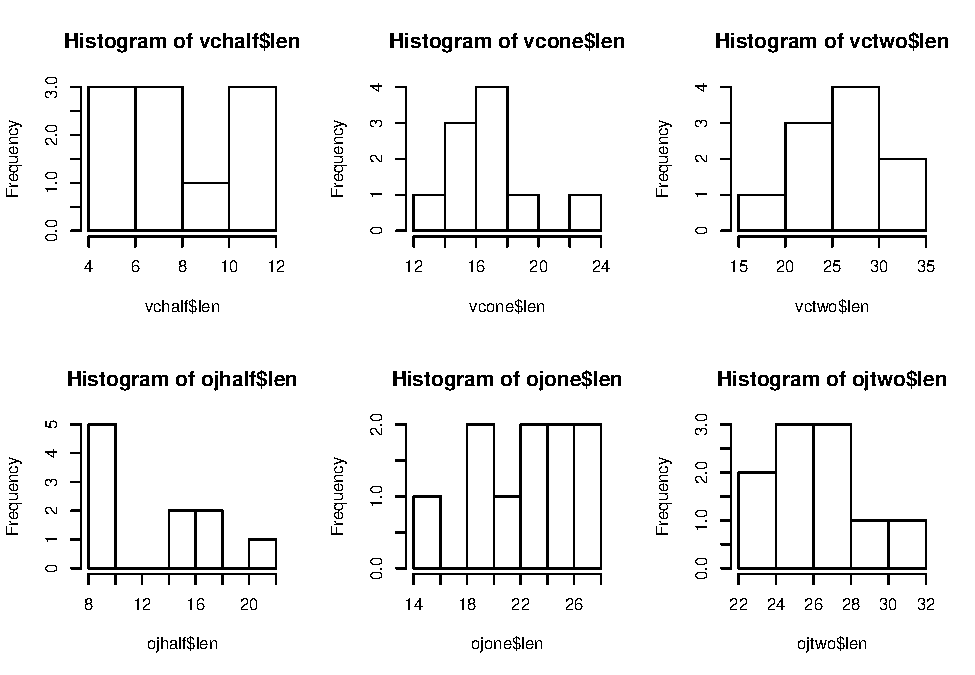
\includegraphics{Final_project_files/figure-latex/unnamed-chunk-1-1.pdf}

The distribution of averages of 40 exponentials can be ploted by

\begin{Shaded}
\begin{Highlighting}[]
\NormalTok{    mns <-}\StringTok{ }\OtherTok{NULL}
    \ControlFlowTok{for}\NormalTok{ (i }\ControlFlowTok{in} \DecValTok{1}\OperatorTok{:}\DecValTok{1000}\NormalTok{)\{}
\NormalTok{      mns <-}\StringTok{ }\KeywordTok{c}\NormalTok{(mns,}\KeywordTok{mean}\NormalTok{(}\KeywordTok{rexp}\NormalTok{(}\DecValTok{40}\NormalTok{,lambda)))}
\NormalTok{    \}}
\NormalTok{    mn <-}\StringTok{ }\KeywordTok{mean}\NormalTok{(mns)}
\NormalTok{    sd <-}\StringTok{ }\KeywordTok{sd}\NormalTok{(mns)}
    
    \KeywordTok{hist}\NormalTok{(mns,}\DataTypeTok{freq =} \OtherTok{FALSE}\NormalTok{)}
    \KeywordTok{curve}\NormalTok{(}\KeywordTok{dnorm}\NormalTok{(x,}\DataTypeTok{mean=}\NormalTok{mn,}\DataTypeTok{sd=}\NormalTok{sd),}\DataTypeTok{col=}\StringTok{"darkblue"}\NormalTok{, }\DataTypeTok{lwd=}\DecValTok{2}\NormalTok{, }\DataTypeTok{add=}\OtherTok{TRUE}\NormalTok{)}
    \KeywordTok{abline}\NormalTok{(}\DataTypeTok{v =}\NormalTok{ mn, }\DataTypeTok{col=}\StringTok{"blue"}\NormalTok{, }\DataTypeTok{lwd=}\DecValTok{3}\NormalTok{)}
    \KeywordTok{text}\NormalTok{(mn}\FloatTok{+0.3}\NormalTok{,}\FloatTok{0.05}\NormalTok{,}\StringTok{"mean"}\NormalTok{)}
    \KeywordTok{abline}\NormalTok{(}\DataTypeTok{v =}\NormalTok{ mn}\OperatorTok{-}\NormalTok{sd, }\DataTypeTok{col=}\StringTok{"red"}\NormalTok{, }\DataTypeTok{lwd=}\DecValTok{3}\NormalTok{)}
    \KeywordTok{text}\NormalTok{(mn}\OperatorTok{-}\NormalTok{sd,}\FloatTok{0.5}\NormalTok{,}\StringTok{"mean-sd"}\NormalTok{)}
    \KeywordTok{abline}\NormalTok{(}\DataTypeTok{v =}\NormalTok{ mn}\OperatorTok{+}\NormalTok{sd, }\DataTypeTok{col=}\StringTok{"red"}\NormalTok{, }\DataTypeTok{lwd=}\DecValTok{3}\NormalTok{)}
    \KeywordTok{text}\NormalTok{(mn}\OperatorTok{+}\NormalTok{sd,}\FloatTok{0.5}\NormalTok{,}\StringTok{"mean+sd"}\NormalTok{)}
\end{Highlighting}
\end{Shaded}

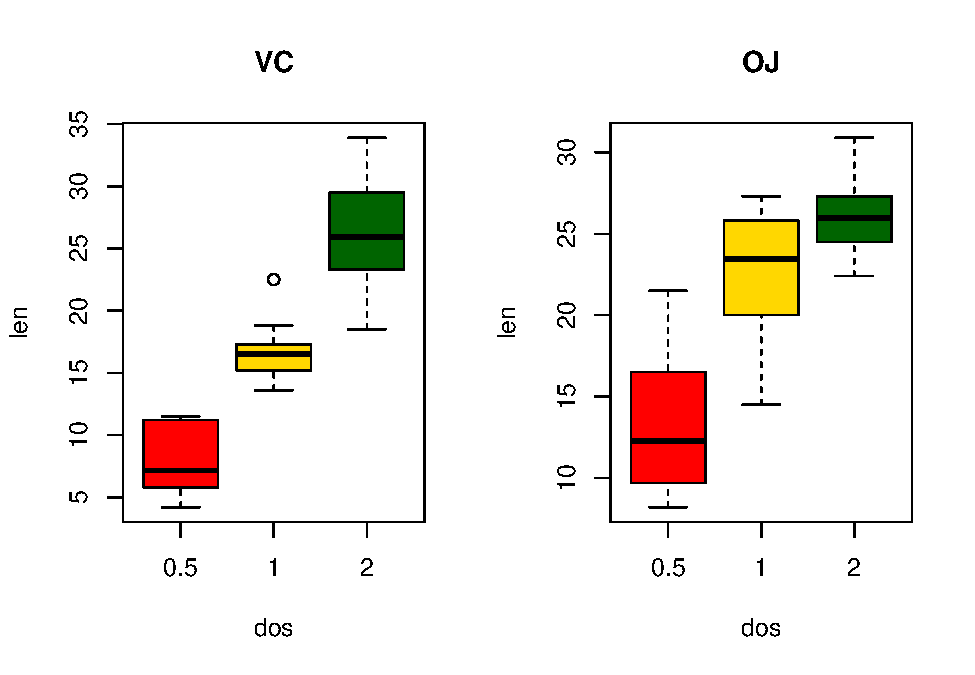
\includegraphics{Final_project_files/figure-latex/unnamed-chunk-2-1.pdf}

The theoretical mean is 1/lambda which is 5, and the sample mean is

\begin{Shaded}
\begin{Highlighting}[]
   \KeywordTok{mean}\NormalTok{(mns)}
\end{Highlighting}
\end{Shaded}

\begin{verbatim}
## [1] 5.025081
\end{verbatim}

which is the thick blue bar in the above figure.

The theoretical standard deviation is also 1/lambda which is 5, so the
theoretical variance is 25. The sample variance and standard deviation
are

\begin{Shaded}
\begin{Highlighting}[]
  \KeywordTok{var}\NormalTok{(mns)}
\end{Highlighting}
\end{Shaded}

\begin{verbatim}
## [1] 0.6094017
\end{verbatim}

\begin{Shaded}
\begin{Highlighting}[]
  \KeywordTok{sd}\NormalTok{(mns)}
\end{Highlighting}
\end{Shaded}

\begin{verbatim}
## [1] 0.7806418
\end{verbatim}

respectively.

The standard deviation is showed in two red lines with the left being
mean-sd and right being mean+sd.

The distribution is closely to a Gaussian distribution which can be seen
from the figure since the histogram overlay with the gaussion
distribution well.

\end{document}
